%%%%%%
% Metadata
%%%%%%

\chapter{Development of the Alpha Recommendation System}
\label{chapter:development}

The main contribution of this thesis is the development of a data driven system for recommending study specific significance levels. Unlike conventional approaches that rely on fixed thresholds such as $\alpha = 0.05$, the proposed system combines empirical evidence from replication studies with machine learning and contextual statistical adjustments. This approach allows the recommended significance level to adapt to study characteristics and research preferences.

This chapter describes how the proposed Alpha Recommendation System is developed. The aim is to address the research gap identified in the previous chapters \ref{sec:litlmitiations} by developing a practical and usable system.

This chapter explains step by step how the final alpha recommendation is generated. It starts with how the data are collected and prepared. Then it explains how the optimal alpha values are defined and how the prediction model is built. After that, it describes how user preferences and contextual adjustments are applied to produce the final recommended alpha. The recommended alpha is not a universal value but is tailored to the specific situation of the user’s study. Together, these steps show how the system works from start to finish.

\section{Overview of the System Design}
\label{sec:overview}
 The purpose of the system is to support researchers in selecting an appropriate significance level ($\alpha$) for hypothesis testing. Instead of relying on a fixed conventional value such as $\alpha = 0.05$, the system provides a recommended $\alpha$ value based on study characteristics and research context. The recommendation is intended to guide decision making during the study design stage and does not replace statistical judgment.

The system is implemented as a software application in Python and 
includes a machine learning component. It operates in two stages: 
a data driven regression model first estimates a baseline significance 
level ($\alpha_{base}$) from sample size and effect size, and a context 
adjustment step then refines this value based on researcher preferences. 
The two stages are described in detail in Sections~\ref{sec:datadriven} 
and~\ref{sec:contextadjust} respectively, and the full system 
architecture is illustrated in Figure~\ref{fig:alpha-flow}.



%\cite{Herzog2019} - about multiple test
%\cite{Akomodi2025} - type 1 type 2 , sample size etc.
%\cite{Baker2016} - lower alpha lower risk dont have acess but mentioned in akomodi
%\cite{Hales2023} - one tailed test
%\cite{Kim2015} - most test use 0.05 and other ways to explore alpha
%\cite{FosterDeardorff2017} - osf is legit
 The overall structure of the Alpha Recommendation System is illustrated in Figure~\ref{fig:alpha-flow}.


\begin{figure}[!ht]
	\centering
	\begin{tikzpicture}[
		>=Stealth,
		every node/.style={align=center, font=\small},
		box/.style={rectangle, draw, rounded corners, minimum width=3.5cm, minimum height=1cm}
		]
		
		% ======================
		% Top Input
		% ======================
		
		\node[box] (input) {Inputs};
		
		\coordinate (split1) at ($(input.south)+(0,-0.8cm)$);
		\draw[->] (input.south) -- (split1);
		
		\coordinate (left1) at ($(split1)+(-3cm,0)$);
		\coordinate (right1) at ($(split1)+(3cm,0)$);
		\draw (left1) -- (right1);
		
		\node[box, below=1.2cm of left1] (sample) {Sample Size};
		\node[box, below=1.2cm of right1] (effect) {Effect Size};
		
		\draw[->] (left1) -- (sample.north);
		\draw[->] (right1) -- (effect.north);
		
		% Merge top
		\coordinate (downsample) at ($(sample.south)+(0,-0.8cm)$);
		\coordinate (downeffect) at ($(effect.south)+(0,-0.8cm)$);
		\coordinate (merge1) at ($(downsample)!0.5!(downeffect)$);
		
		\draw (sample.south) -- (downsample);
		\draw (downsample) -- (merge1);
		
		\draw (effect.south) -- (downeffect);
		\draw (downeffect) -- (merge1);
		
		% ======================
		% Stage 1 + Baseline
		% ======================
		
		\node[box, below=1.5cm of merge1] (model)
		{Stage 1: Data-Driven Model (Regression)};
		
		\draw[->] (merge1) -- (model.north);
		
		\node[box, below=1.3cm of model] (base)
		{Baseline Alpha ($\alpha_{base}$)};
		
		\draw[->] (model) -- (base);
		
		\node[box, below=1.3cm of base] (context)
		{Stage 2: Context Adjustment};
		
		\draw[->] (base) -- (context);
		
		% ======================
		% Bottom Split (3-way)
		% ======================
		
		\coordinate (split2) at ($(context.south)+(0,-0.8cm)$);
		\draw[->] (context.south) -- (split2);
		
		\coordinate (left2) at ($(split2)+(-5.0cm,0)$);
		\coordinate (mid2) at ($(split2)+(0,0)$);
		\coordinate (right2) at ($(split2)+(5.0cm,0)$);
		
		\draw (left2) -- (right2);
		
		\node[box, below=1.2cm of left2] (risk) {Risk Tolerance};
		\node[box, below=1.2cm of mid2] (test) {Test Direction};
		\node[box, below=1.2cm of right2] (num) {Number of Tests};
		
		\draw[->] (left2) -- (risk.north);
		\draw[->] (mid2) -- (test.north);
		\draw[->] (right2) -- (num.north);
		
		% Merge bottom
		\coordinate (downrisk) at ($(risk.south)+(0,-0.8cm)$);
		\coordinate (downtest) at ($(test.south)+(0,-0.8cm)$);
		\coordinate (downnum) at ($(num.south)+(0,-0.8cm)$);
		
		\coordinate (merge2) at ($(downrisk)!0.5!(downnum)$);
		
		\draw (risk.south) -- (downrisk);
		\draw (downrisk) -- (merge2);
		
		\draw (test.south) -- (downtest);
		\draw (downtest) -- (merge2);
		
		\draw(num.south) -- (downnum);
		\draw (downnum) -- (merge2);
		
		% ======================
		% Final Alpha
		% ======================
		
		\node[box, below=1.5cm of merge2] (final)
		{Final Recommended Alpha ($\alpha_{final}$)};
		
		\draw[->] (merge2) -- (final.north);
		
	\end{tikzpicture}
	\caption{Flow diagram of the Alpha Recommendation System.}
	\label{fig:alpha-flow}
\end{figure}




\subsection{Data Driven Alpha Recommendation}
\label{sec:datadriven}
The first stage of the Alpha Recommendation System predicts a baseline value for the significance level ($\alpha$) using information from past replication studies. This stage relies only on information that is available before performing the hypothesis test for the new study.

Two inputs are used: sample size and effect size. These variables are chosen because they are specified during study planning and influence statistical power and error rates\cite{PetersonFoley2021}. No $p$-values or results from the new study are used at this stage.

Replication data are used to examine how different combinations of sample size and effect size are associated with appropriate $\alpha$ values in previous studies. Based on these patterns, the system learns a general relationship between these inputs and corresponding alpha values.

When a researcher provides the sample size and expected effect size for a new study, the system applies this learned relationship to produce a baseline $\alpha$ value. This value reflects patterns observed in similar past studies and serves as a starting point rather than a final decision.

The internal data preparation and model training procedure used to obtain this $\alpha_{base}$ value are described in a later sections \ref{sec:Dataset} and \ref{sec:MLpart}.

\subsection{Context Based Adjustment of Alpha}
\label{sec:contextadjust}
The $\alpha_{base}$ value produced in the first stage does not include all aspects of a study. Accurate decisions depend on the research context and the researcher’s preferences in addition to the patterns observed in replication data which provide only a numerical baseline and do not account for the specific context or preferences of the researcher. For this reason, the Alpha Recommendation System includes a second stage that adjusts the $\alpha_{base}$ value using user defined inputs.

In this stage, the user provides information about the study context. Three factors are considered: risk tolerance, test directionality (one tailed or two tailed), and the number of hypotheses being tested. These factors were selected because they are commonly used in classical hypothesis testing and have a clear connection to the choice of the significance level.

The system applies simple and predefined rules to modify the $\alpha_{base}$ value. Stricter risk preferences lead to smaller $\alpha$ values, while more lenient preferences allow larger values\cite{Baker2016}.

The first adjustment modifies the baseline alpha according to the selected level of risk tolerance
\begin{equation}
	\alpha' 
	= 
	\alpha_{\text{base}} \cdot k_1
\end{equation}
where $\alpha'$ denotes the risk-adjusted baseline alpha and 
$k_1$ is the risk tolerance scaling factor.
One tailed tests and multiple hypothesis testing are handled using standard statistical adjustments.
 
The second adjustment accounts for the structural difference between one tailed and two tailed tests\cite{Hales2023}:
 \begin{equation}
 	\alpha'' =
 	\begin{cases}
 		2\alpha' & \text{if one-tailed} \\
 		\alpha'  & \text{if two-tailed}
 	\end{cases}
 \end{equation}
 where $\alpha''$ denotes the directionality adjusted alpha value.
This adjustment reflects the allocation of the rejection region in hypothesis testing.

Finally, when multiple hypotheses are tested simultaneously, a Bonferroni-style correction is applied\cite{Herzog2019}:
\begin{equation}
	\alpha_{\text{final}} 
	= 
	\frac{\alpha''}{m}
\end{equation}
where m denotes the number of hypothesis tests conducted.

To ensure numerical stability and interpretability, the final alpha value is restricted to the interval:

This prevents unrealistically small or excessively large significance levels.

\begin{equation}
	0.001 \leq \alpha_{\text{final}} \leq 0.15
	\label{eq.alpharange}
\end{equation}

The rules are transparent, so the effect of each input on the final $\alpha$ value is easy to understand.

Although only three contextual factors are included, the system remains broadly usable. The $\alpha_{base}$ value, which is derived from replication data, can serve as a default and data informed reference for selecting the significance level. The contextual adjustments are optional refinements that allow the recommendation to better reflect specific study preferences. Even if additional contextual factors are not included, the system still provides a more flexible and evidence based alternative to using a fixed value such as $\alpha = 0.05$.
The overall adjustment process can be summarized mathematically as follows:

\begin{equation}
	\alpha_{\text{final}} 
	= 
	\alpha_{\text{baseline}} 
	\cdot k_1 
	\cdot k_2 
	\cdot k_3
\end{equation}

where $k_1$ represents the risk preference factor, 
$k_2$ represents the test direction factor, 
and $k_3$ represents the multiple testing correction factor.
After applying the adjustments, the system produces a final recommended $\alpha$ value. This value is selected before conducting the hypothesis test and does not depend on observed data or $p$-values. It does not replace statistical judgment, but instead provides a structured and context aware reference for choosing the significance level.

The implementation details used to perform these adjustments are described in the following section.

\section{Dataset Construction and Optimal Alpha Definition}
\label{sec:Dataset}
This section explains how the dataset used in the Alpha Recommendation System is constructed. It describes the data sources, their reliability, the procedure used to define optimal alpha values, the methods used to recover missing sample sizes and effect sizes, and the structure of the final dataset.

The dataset used in the Alpha Recommendation System is constructed by combining results from several large scale replication projects available through the Open Science Framework (OSF). These projects report findings from original studies together with the results of independent replication attempts across multiple research fields\cite{FosterDeardorff2017}. Each row in the final dataset represents a single hypothesis test.

In many original studies, the significance level ($\alpha$) is not explicitly reported. This is because most studies follow the common convention of using $\alpha = 0.05$\cite{Kim2015}. When a different significance level is used, it is usually stated clearly in the study. Therefore, when no $\alpha$ value is reported, it is assumed that the original study used $\alpha = 0.05$. This assumption reflects common reporting practice in empirical research.

For studies in which the replication confirms the original finding, the significance level used in the original study is treated as appropriate. In these cases, the original $\alpha$ value (either reported or assumed to be 0.05) is recorded as the optimal alpha, since the original decision is supported by the replication outcome.

For studies in which the replication does not confirm the original finding, the original significance level is considered too lenient. In such cases, an alternative $\alpha$ value is calculated using the original study’s reported $p$-value. The purpose is to determine which significance level would have led to a correct decision when compared with the replication result. The optimal alpha is defined as the largest significance level that is smaller than the original $p$-value. This ensures that the original result would not have been declared statistically significant under the adjusted threshold. The calculations are explained in detail in Section \ref{subsec:OAlphaCalculation}.

This procedure generates a study specific optimal alpha value for each hypothesis test in the dataset. The calculation relies only on information reported in the original and replication studies, including $p$-values, test statistics, sample size, and effect size. When necessary, standard statistical relationships are used to ensure consistency across different study designs.

After applying this procedure to all replication projects, the result is a single combined dataset in which each row represents one hypothesis test and includes a clearly defined optimal alpha value. This optimal alpha serves as the target variable for the data driven component of the Alpha Recommendation System. The detailed steps of dataset construction and the full procedure for defining the optimal alpha are explained in the following sections.

\subsection{Data Acquisition}

The dataset used in this study is constructed by combining results from five large scale replication projects available on the Open Science Framework (OSF). These projects report findings from original studies together with the results of independent replication attempts across multiple research domains\cite{FosterDeardorff2017}. Each row in the final dataset used in this project represents a single hypothesis test.


	{\renewcommand{\arraystretch}{1.35}
\begin{table}[H]
	\centering
	\caption{Overview of replication projects included in the dataset}
	\resizebox{\textwidth}{!}{
		\begin{tabular}{p{5cm} p{3cm} p{8cm}}
			\toprule
			\textbf{Replication Project} & \textbf{Research Field} & \textbf{Main Variables Extracted} \\
			\midrule
			
			Reproducibility Project: Cancer Biology \cite{ErringtonDenis2021}
			& Biomedical 
			& Original $p$-values, standardized effect sizes, sample sizes, and replication $p$-values. \\
			
			Challenging the N-Myopia\cite{Li2021} 
			& Psychology 
			& Original $p$-values, effect sizes, sample sizes, and replication success indicators. \\
			
			Applying Z-Curve to Large-Scale Replication Studies \cite{Sotola2022}
			& Psychology 
			& Effect sizes and sample sizes derived from reported test statistics together with replication outcomes. \\
			
			Pre-hacking Project\cite{Chang2025} 
			& Psychology 
			& Original $p$-values, recovered effect sizes, sample sizes, and replication results. \\
			
			Life Outcomes of Personality Replication (LOOPR)\cite{Soto2017} 
			& Personality / Outcomes 
			& Preregistered effect sizes, sample sizes, and replication outcomes. \\
			
			\bottomrule
		\end{tabular}
	}
	
	\label{tab:replication_projects}
\end{table}

\subsection{Data Quantity}

After cleaning and compilation, the final dataset contains 664 individual hypothesis tests drawn from five replication projects. The contributions from each project are as follows:

\begin{itemize}
	\item Cancer Biology Replication Project: 135 tests
	\item N-Myopia Replication Project: 310 tests
	\item Z-Curve Replication Studies: 136 tests
	\item LOOPR Replication Project: 75 tests
	\item Pre-hacking Replication Project: 8 tests
\end{itemize}

Combining multiple replication projects increases diversity in study design and reduces reliance on a single research domain. Sample sizes in the dataset range from very small studies to large scale experiments with sample sizes exceeding 200,000. Effect sizes also cover a wide range, including both small and large effects.

The size of the dataset is sufficient for the purpose of this study because the goal is not high dimensional prediction, but learning stable relationships between a small number of predictors—primarily sample size and effect size—and corresponding optimal alpha values. The dataset provides adequate variation across study contexts while remaining manageable and interpretable.

\subsection{Data Quality and Reliability}

The Open Science Framework is widely used for sharing replication data because it promotes transparency and open research practices. Replication studies hosted on OSF are typically conducted by independent research teams, often follow preregistered analysis plans, and provide open access to data and study materials, replication projects hosted on OSF are conducted by established research teams and are published in peer reviewed journals, which ensures that the results have been scientifically reviewed and validated\cite{FosterDeardorff2017}. These characteristics increase the credibility of the replication outcomes and make OSF projects a reliable source for evaluating statistical decision rules such as hypothesis testing.

The selected projects cover different research fields, including psychology, behavioral science, personality research, and biomedical science. This cross disciplinary selection ensures diversity in study designs and increases the generalizability of the constructed dataset. Each project provides hypothesis level information including $p$-values, effect sizes, sample sizes, and replication outcomes.

\subsection{Data Relevance}

Replication data are directly relevant because they allow evaluation of whether original statistical decisions were supported by subsequent evidence\cite{FosterDeardorff2017}. By linking original $p$-values, sample sizes, effect sizes, and replication outcomes, the dataset provides a structured basis for analyzing how different significance levels relate to reproducibility..

\subsection{Handling Missing Values and Anomalies}

Not all studies reported complete information. Some studies did not explicitly report sample size or effect size but provided test statistics such as $t$, $F$, or $\chi^2$ values. Rather than discarding these studies, standard statistical relationships were used to recover missing quantities when sufficient information was available. The methods are explained in \ref{subsec:SampleEfeectCalc}

Studies that lacked enough information to reliably recover sample size or effect size were excluded. No aggressive outlier removal was applied. Only clearly implausible or incomplete records were removed to maintain consistency while preserving as much valid replication information as possible.

\subsection{Definition and Calculation of Optimal Alpha}
\label{subsec:OAlphaCalculation}
In some original studies, the significance level ($\alpha$) used for hypothesis testing is not explicitly reported. This is because most studies follow the conventional choice of $\alpha = 0.05$ \cite{Kwak2023}. When an alternative significance level is used, authors typically report it explicitly. Therefore, when no $\alpha$ value is reported, it is assumed that the original study used $\alpha = 0.05$.
%\cite{Kwak2023} - states most studies use 0.05
For studies in which the replication successfully confirms the original finding, the original significance level is treated as appropriate. In these cases, the original $\alpha$ value (reported or assumed) is recorded as the optimal alpha, since the original decision is supported by the replication outcome.

For studies in which the replication does not confirm the original finding, 
the original significance level is considered too lenient.Concerns 
about overly permissive significance thresholds and their impact on 
replication have been widely discussed in the statistical literature 
\cite{Benjamin2018, WassersteinLazar2016}. In such cases, 
an alternative significance level is derived using the original study's 
reported $p$-value $p_{\text{orig}}$. The objective is to determine a 
study specific significance level that would have resulted in a 
non significant outcome in the original study while remaining as close as 
possible to the reported $p$-value.

Concretely, the optimal alpha is defined as

\begin{equation}
	\alpha_{\text{opt}} = \max \{ \alpha \in \mathcal{A} : \alpha < p_{\text{orig}} \},
\end{equation}
\label{eq:optalpha}
where 

\[
\mathcal{A} = \{0.001,\,0.005,\,0.01,\,0.02,\,0.03,\,0.04,\,0.05,\,0.06,\,0.09,\,0.10\}
\]
This candidate set was derived empirically from the replication 
dataset. The optimal alpha values observed across all 664 studies 
fell within this discrete range, making these values the natural 
choice for the candidate set.

This Formula\ref{eq:optalpha} was derived specifically for this system to operationalise 
the concept of a study-specific threshold. While the general idea of 
adapting significance levels to study outcomes is discussed in the 
literature \cite{Benjamin2018}\cite{WassersteinLazar2016}, the 
specific formulation presented here was developed as part of this work.

is a predefined set of candidate significance levels. This rule ensures that 
the original result would not have been declared statistically significant 
under $\alpha_{\text{opt}}$, while the chosen value remains interpretable 
and comparable across studies.

For example, if a study has $p = 0.047$ and the replication did not find the effect, using $\alpha = 0.05$ would incorrectly declare the result significant. Using $\alpha = 0.04$ would correctly declare it non significant. In this case, $\alpha = 0.04$ is the optimal alpha for that study.

This procedure produces a study specific optimal alpha value for every hypothesis test in the dataset. The optimal alpha serves as the target variable for the data driven component of the Alpha Recommendation System.

\textbf{It is important to note that replication outcomes alone cannot determine a theoretically optimal significance level. The procedure used here should therefore be interpreted as a pragmatic approximation. Similar discussions about adapting significance thresholds in response to replication evidence can be found in the statistical literature on reproducibility and significance testing \cite{Benjamin2018, WassersteinLazar2016, OpenScience2015}.}

\subsection{Derivation of Sample Size and Effect Size}
\label{subsec:SampleEfeectCalc}
To ensure consistency across studies, each hypothesis test must be associated with a sample size and an effect size. When these values were not reported directly, they were recovered using standard statistical formulas.

For $t$-tests with reported degrees of freedom, effect size $r$ was computed as \cite{becker2000}:

\begin{equation}
	r = \sqrt{\frac{t^2}{t^2 + df}}
\end{equation}

If sample size was not explicitly reported but degrees of freedom were available, sample size was recovered as\cite{Cohen1988}:

\begin{equation}
	N = df + 2
\end{equation}

For $\chi^2$ tests with one degree of freedom, effect size was computed using \cite{kim2017}:

\begin{equation}
	\phi = \sqrt{\frac{\chi^2}{N}}
\end{equation}

For $F$-tests with one numerator degree of freedom, effect size was computed as \cite{RICHARDSON2011}:

\begin{equation}
	\eta^2 = \frac{F \cdot df_1}{F \cdot df_1 + df_2},
	\qquad
	r = \sqrt{\eta^2} 
\end{equation}

Only studies for which both sample size and effect size could be reliably obtained were retained. A complete list of formulas is provided in Appendix~A.

\subsection{Final Dataset Structure}

After combining replication projects, computing optimal alpha values, and recovering missing sample sizes and effect sizes, the final dataset consists of standardized rows. Each row represents one hypothesis test.

Table~\ref{tab:dataset_example} shows the first five rows of the final dataset to illustrate its structure.

\begin{table}[ht]
	\centering
	\caption{First Five Rows of the Final Dataset}
	\label{tab:dataset_example}
	\begin{tabular}{cccc}
		\hline
		Sample Size & Effect Size & Replication Success & Best Alpha \\
		\hline
		30   & 0.18 & 0 & 0.031 \\
		120  & 0.25 & 1 & 0.050 \\
		85   & 0.14 & 0 & 0.042 \\
		300  & 0.36 & 1 & 0.050 \\
		1000 & 0.62 & 0 & 0.090 \\
		\hline
	\end{tabular}
\end{table}

The final dataset is used as input for the machine learning component of the Alpha Recommendation System. Sample size and effect size are used as predictors, and optimal alpha is used as the target variable.

It should be noted that larger sample sizes do not always 
correspond to stricter optimal $\alpha$ values in the dataset. 
In cases where the effect size is relatively large and the 
original $p$-value was substantially above a conventional 
threshold, the calculated optimal $\alpha$ may exceed $0.05$ 
even when the replication failed. This reflects the specific 
$p$-value reported in the original study rather than a general 
recommendation for leniency.

\section{ML Model for Predicting $\alpha_{base}$ }
\label{sec:MLpart}
This section explains how the constructed dataset is processed specifically for model training, how the input features and target variable are selected, and how the data driven model is implemented to estimate a $\alpha_{base}$.

While the previous section described how the dataset was built and how optimal alpha values were defined\ref{sec:Dataset}, this section focuses on preparing the data for machine learning and implementing the predictive model.

\subsection{Data Preparation for Model Training}

After the dataset is constructed and the optimal alpha values are defined, it is prepared for use in the machine learning model. The purpose of this step is to ensure that the data are suitable for training while preserving the original information as much as possible.

Only rows that contain all required variables are retained. Each observation must include:

\begin{itemize}
	\item Valid sample size,
	\item  Valid effect size,
	\item  Defined optimal alpha value.
\end{itemize}

Rows are removed only when essential information is missing and cannot be recovered. For example, if sample size or effect size cannot be derived from the available statistics, that observation is excluded.

Clearly invalid values are also removed. Observations with zero or negative sample sizes, undefined effect sizes, or inconsistent values are excluded to prevent errors during model training.

No additional filtering or transformation is applied beyond these basic checks. Sample sizes are not trimmed, and effect sizes are not rescaled unless required during calculation. This approach preserves the natural variation in the replication data and allows the model to learn from real differences between studies.

After these steps, the dataset contains complete and valid observations suitable for training the predictive model.

\subsection{Feature Selection and Target Variable}

The goal of the model is to recommend a significance level before conducting a hypothesis test. Therefore, only information known at the study design stage is used as input.

Two input features are selected:

\begin{itemize}
	\item Sample size
	\item Effect size
\end{itemize}

Sample size is included because it directly affects statistical power and the balance between Type I and Type II errors. Larger studies can often support stricter significance levels, while smaller studies may require more flexible thresholds \cite{maier2022}.

Effect size is included because it reflects the strength of the expected relationship. Studies targeting small effects face different decision challenges than those targeting larger effects \cite{mudge2012}.

The model predicts the optimal alpha value as a continuous variable. This optimal alpha represents the significance level that would have produced a decision consistent with the replication outcome.

Contextual factors such as risk tolerance, test directionality, and multiple testing are not included in this stage because they are handled in stage two of the application and explained step by step in following sections \ref{sec:ContextFactors}.

\subsection{Conceptual Idea of the Data Driven Model}

The purpose of the data driven model is to estimate a baseline alpha value based on patterns observed in replication studies. The model does not make final decisions about hypothesis testing. Instead, it provides a reference value based on empirical evidence.

Each training example (Each row in the dataset) consists of:

\begin{itemize}
	\item Sample size (input)
	\item Effect size (input)
	\item optimal alpha value (target).
\end{itemize}

The model learns how changes in sample size and effect size are associated with changes in suitable significance levels. If studies with certain characteristics required stricter or more lenient alpha values to align with replication outcomes, the model captures this pattern.

When new study inputs are provided, the model produces a $\alpha_{base}$ value based on pattern learned from similar past cases.


\subsection{Choice of Algorithm}

The predictive model is implemented in Python using the scikit-learn library. Scikit-learn is a widely used open source machine learning library that provides tools for data preprocessing, model training, evaluation, and prediction. It allows the implementation of various machine learning algorithms in a structured and efficient way \cite{scikit-learn2023}.

Since the objective is to predict a continuous optimal alpha value, the problem is formulated as a regression task. A regression algorithm learns a function that maps input variables to a continuous numerical output. Three candidate algorithms were evaluated. A Decision Tree regressor partitions the input space into regions and assigns a constant prediction to each region. A XGBoost regressor builds trees sequentially, where each new tree corrects the residual errors of the previous one. A Random Forest regressor builds a large number of independent decision trees and combines their predictions by averaging, which reduces variance and improves generalization\cite{Breiman2001}. Their predictive performance was compared using standard evaluation metrics \ref{fig:DecisonTree}, \ref{fig:GradientBoosting},\ref{fig:RandomForest}.

To evaluate predictive performance, the dataset was divided into training and testing subsets. Eighty percent of the observations were used to train the models, while the remaining twenty percent were reserved for testing. Model performance was evaluated on the test set using the Mean Absolute Error (MAE) metric.

The Mean Absolute Error (MAE) is defined as

\begin{equation}
	\text{MAE} = \frac{1}{n} \sum_{i=1}^{n} |y_i - \hat{y}_i|
\end{equation}

where $y_i$ represents the true value and $\hat{y}_i$ represents the predicted value\cite{WillmottMatsuura2005}.

\begin{figure}[H]
	\centering
	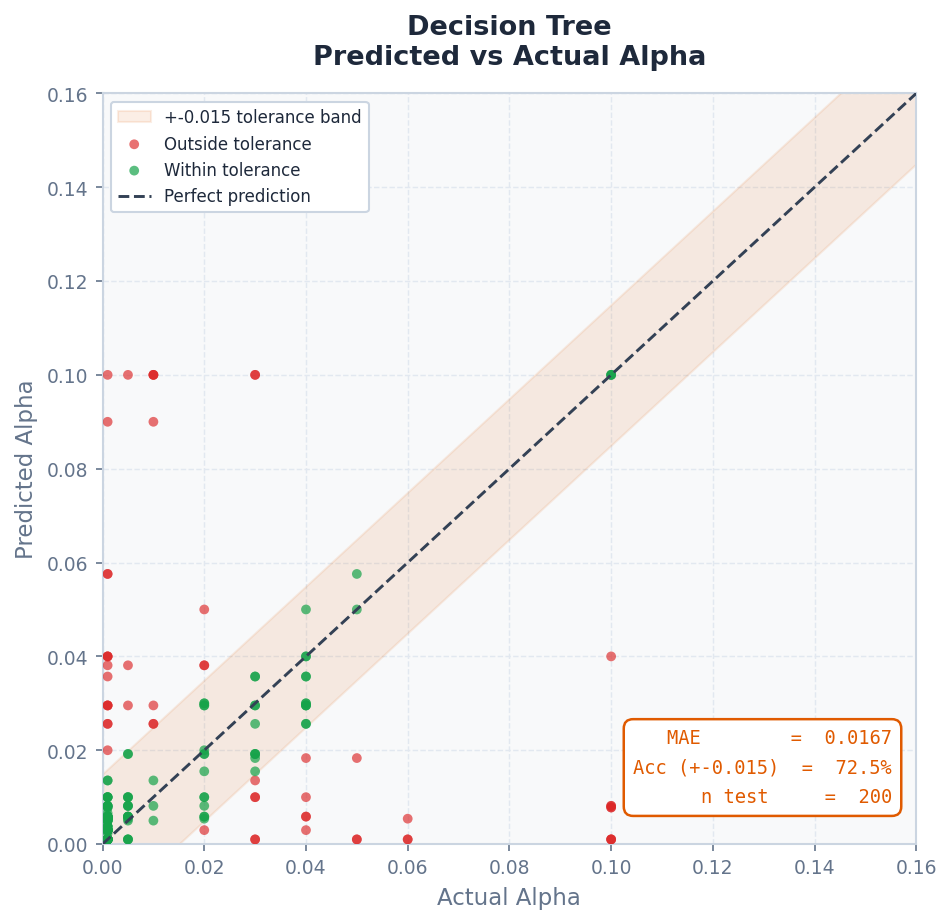
\includegraphics[width=0.7\textwidth]{Images/pred_vs_actual_decision_tree}
	\caption{Decision Tree Regressor: Predicted/Actual Alpha Values }
	\label{fig:DecisonTree}
\end{figure}


\begin{figure}[H]
	\centering
	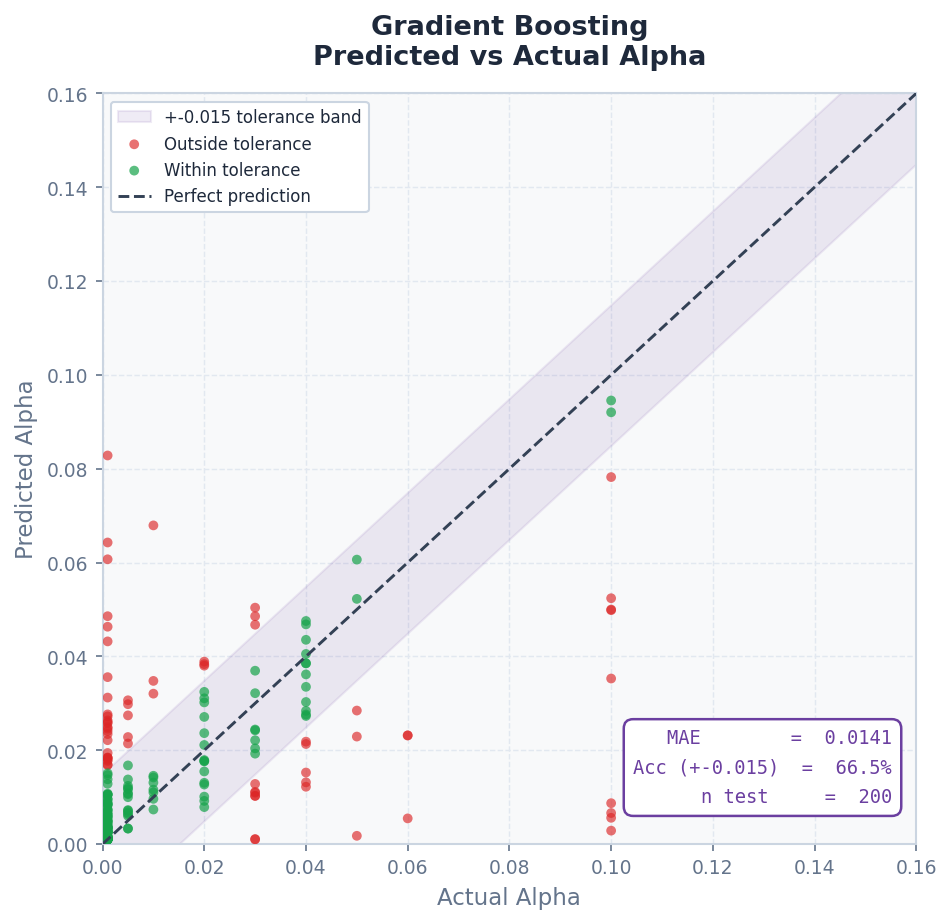
\includegraphics[width=0.7\textwidth]{Images/pred_vs_actual_gradient_boosting}
	\caption{Gradient Boosting Regressor: Predicted/Actual  Alpha Values}
	\label{fig:GradientBoosting}
\end{figure}

\begin{figure}[H]
	\centering
	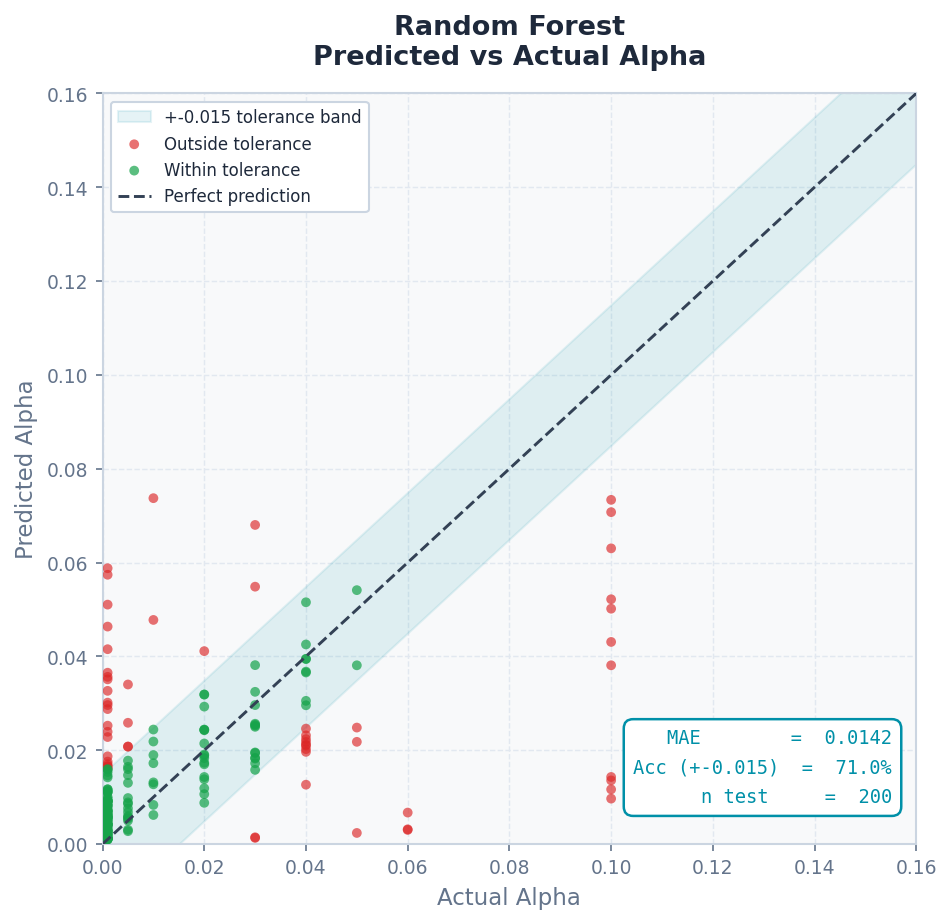
\includegraphics[width=0.8\textwidth]{Images/pred_vs_actual_random_forest}
	\caption{Random Forest Regressor: Predicted/Actual  Alpha Values}
	\label{fig:RandomForest}
\end{figure}

Among the tested models, the Random Forest regression algorithm 
achieved the lowest Mean Absolute Error (MAE) of $0.0142$ on the 
test set ($n = 208$), with $71.0\%$ of predictions falling within 
a $\pm 0.015$ tolerance band. This outperformed the Decision Tree 
($\text{MAE} = 0.0167$, $72.5\%$ within tolerance) and Gradient 
Boosting ($\text{MAE} = 0.0141$, $66.5\%$ within tolerance) 
regressors.

 Random Forest builds multiple decision trees and combines their predictions by averaging  and better explained in Figure\ref{fig:randomforestregressor}\cite{Breiman2001}.
 This approach better
 
 \begin{itemize}
 	\item captures non linear relationships,
 	\item reduces sensitivity to noise,
 	\item and does not require strong distributional assumptions.\cite{Ryo2017}
 \end{itemize}
 
 The objective is not to develop a new algorithm, but to use a reliable and widely accepted method to learn patterns from replication data.
\begin{figure}[htbp]
 	\centering
 	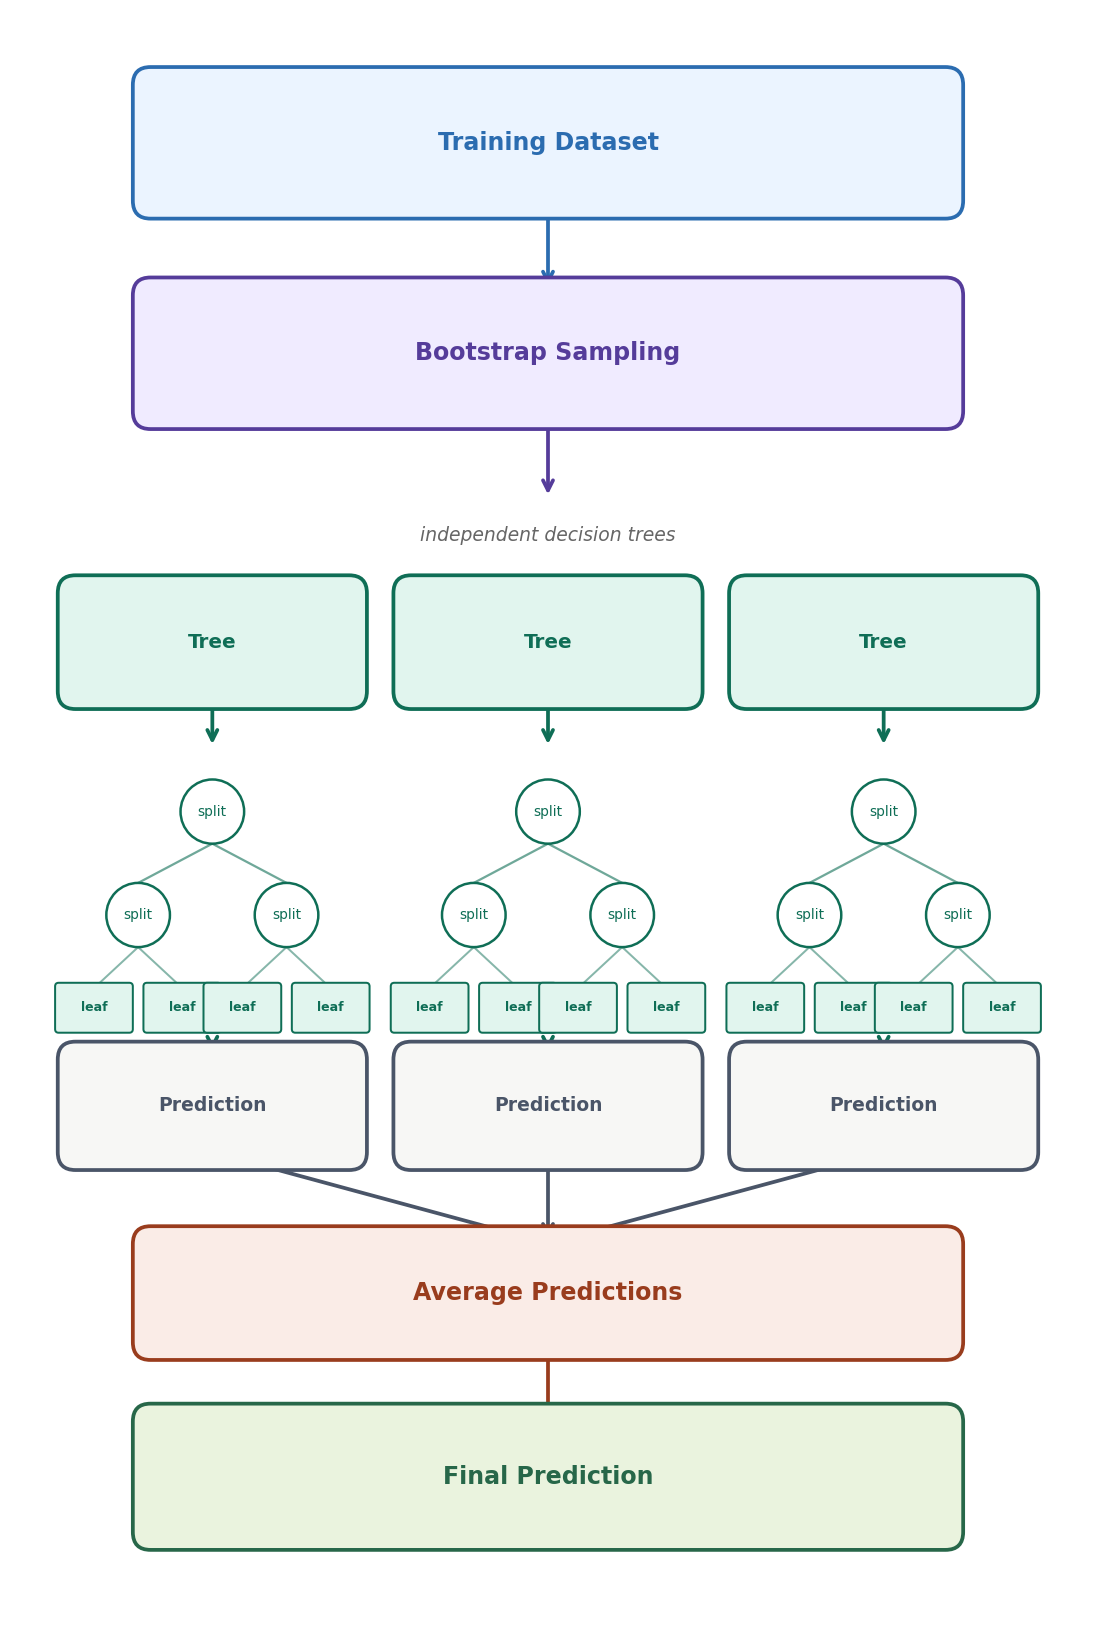
\includegraphics[width=0.8\textwidth]{Images/random_forest_vertical}
 	\caption{Structure of the Random Forest regression model used for predicting the baseline significance level.(based on \cite{Ha2023})}
 	\label{fig:randomforestregressor}
 \end{figure}


The predictive performance of the models was evaluated using the regression metric Mean Absolute Error (MAE). MAE measures the average absolute difference between the predicted and actual values. This metric was chosen because it is easy to understand and expresses the prediction error in the same units as the target variable. In addition, MAE is less sensitive to large errors than metrics such as Mean Squared Error (MSE), since it does not square the differences between predicted and actual values \cite{WillmottMatsuura2005}.
\begin{figure}[htbp]
	\centering
	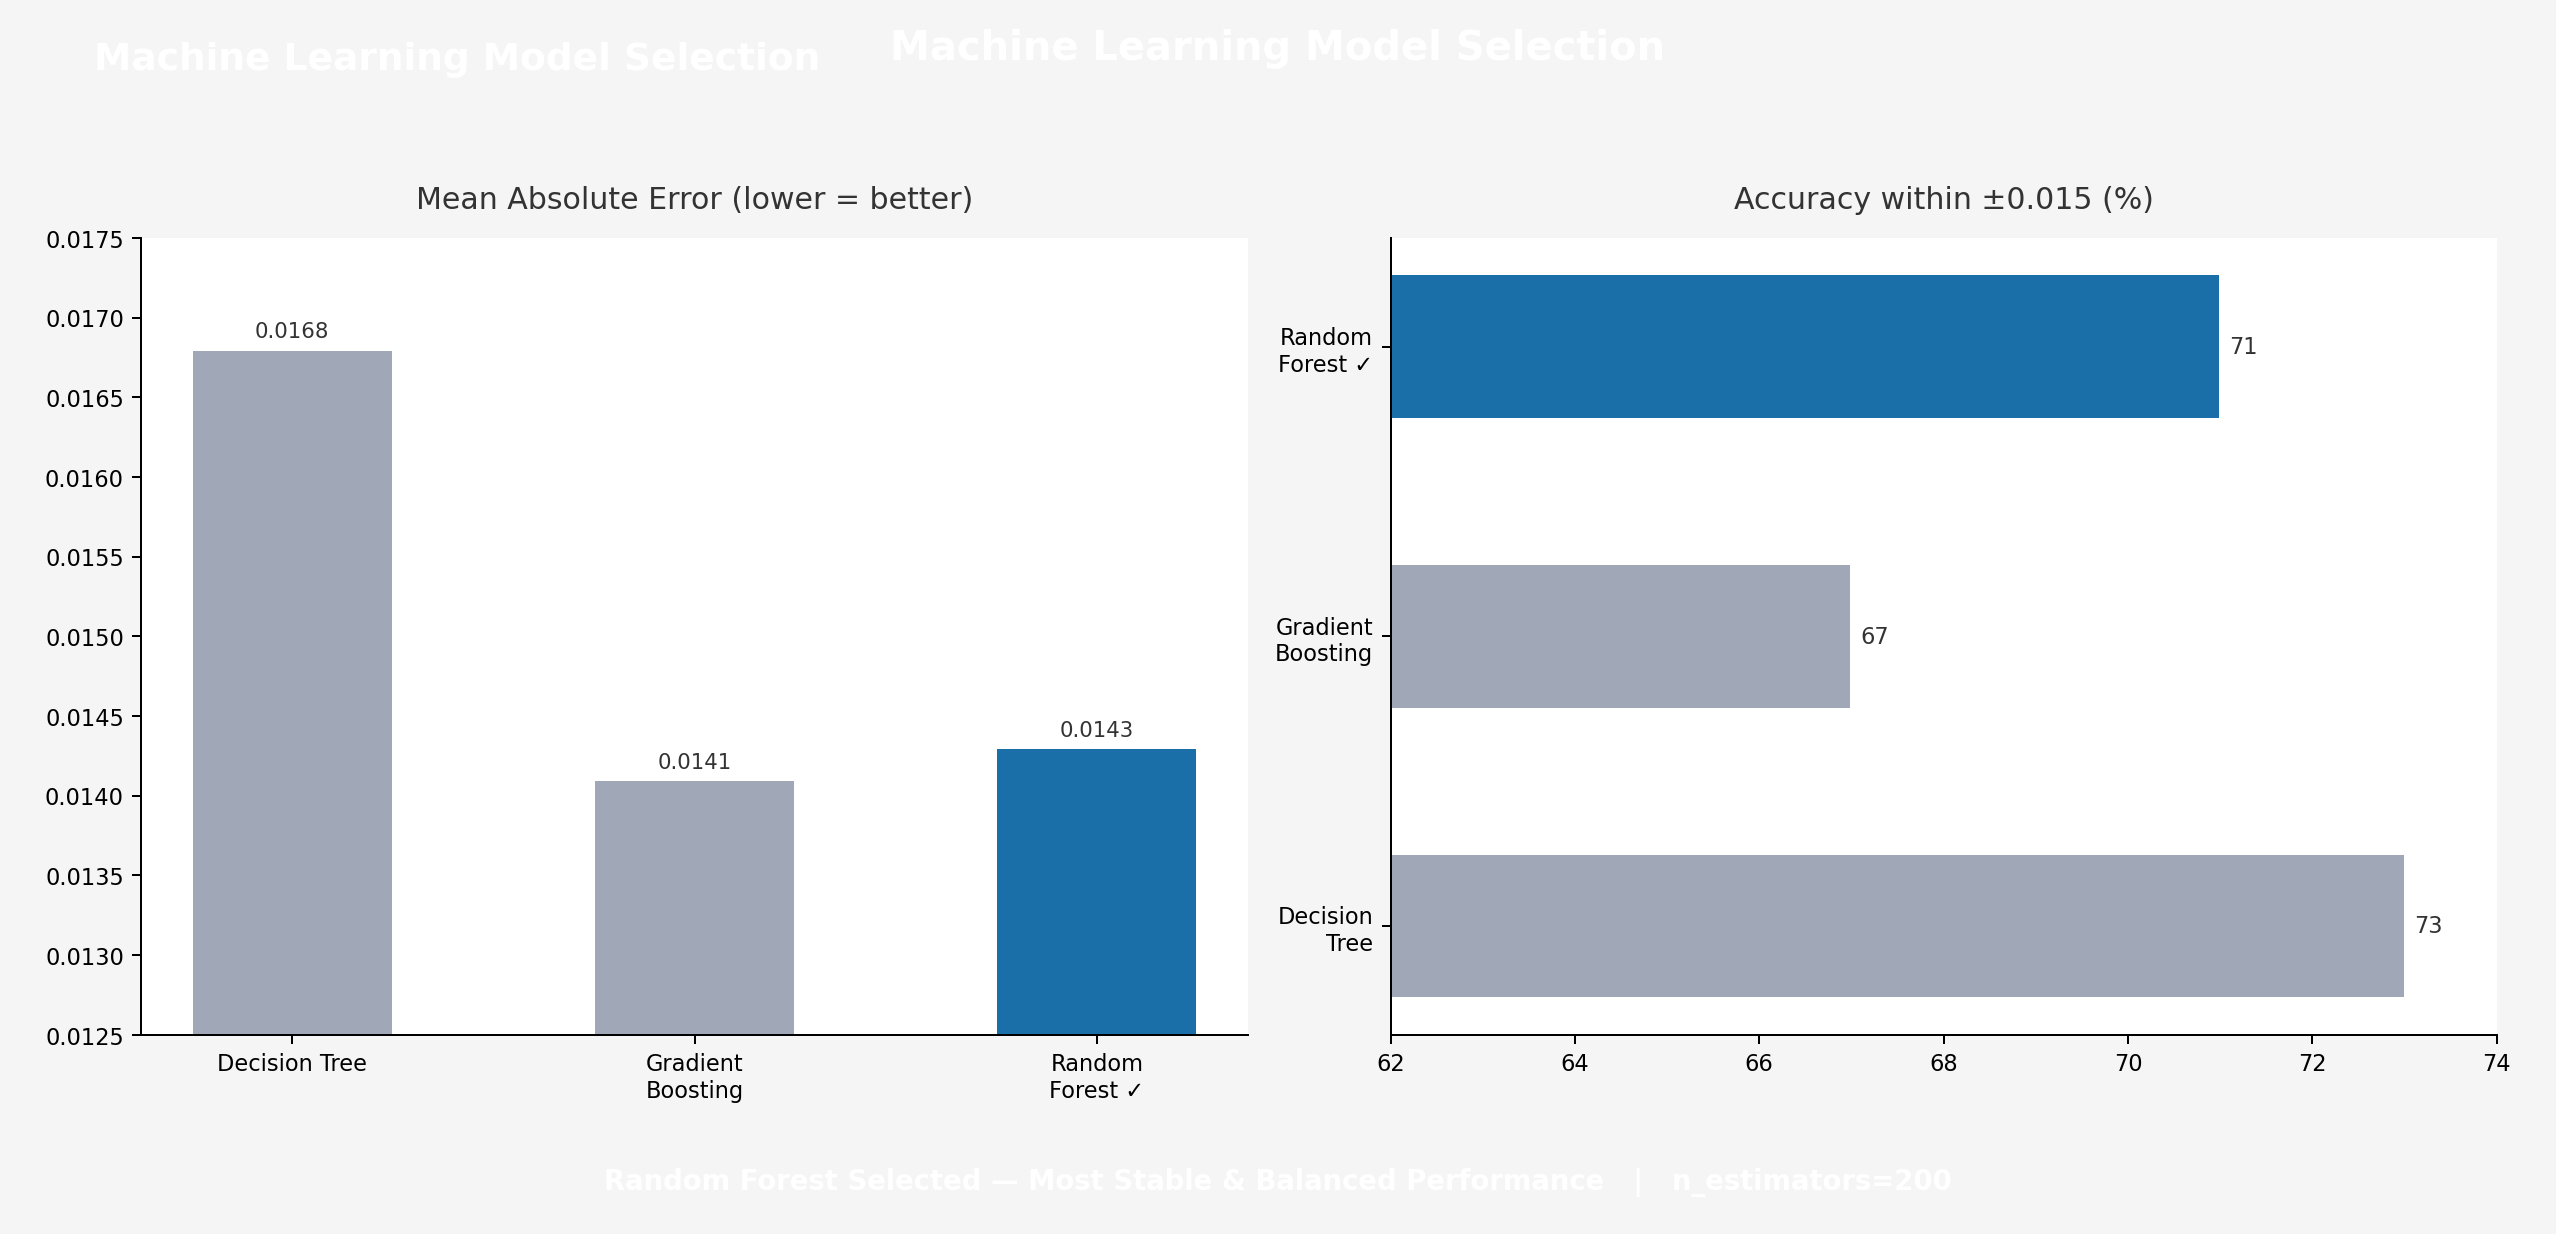
\includegraphics[width=0.7\textwidth]{Images/ml_model_selection}
	\caption{Performance comparison of ML models }
	\label{fig:MLmodelComparision}
\end{figure}

Among the tested models, the Random Forest regression algorithm achieved the lowest MAE\ref{fig:RandomForest}, indicating better predictive performance compared to the alternative models.


\subsection{Model Implementation in Python}

The implementation is written in Python using standard data analysis and machine learning libraries, including \textbf{pandas for data handling, NumPy} for numerical operations, and \textbf{scikit-learn} for model training and evaluation. Each step of the implementation, including data preparation, model training, prediction, and evaluation, is described in detail in the following sections.

\subsubsection*{Loading the Data}

\begin{lstlisting}[language=Python]
	import pandas as pd
	
	data = pd.read_excel("master_alpha_dataset_updated.xlsx")
	
	X = data[["sample_size", "effect_size"]]
	y = data["best_alpha"]
\end{lstlisting}

The dataset is loaded from an Excel file using the pandas library. The variables \textbf{sample size} and \textbf{effect size} are selected as input features (X), and \textbf{best alpha} is selected as the target variable (y). This separation allows the model to learn the relationship between study characteristics and the optimal alpha value.

\subsubsection*{Training the Model}

\begin{lstlisting}[language=Python]
	from sklearn.ensemble import RandomForestRegressor
	
	model = RandomForestRegressor(n_estimators=200, random_state=42)
	model.fit(X, y)
\end{lstlisting}

\subsubsection{Training the Model}

The Random Forest regression model was implemented using the \texttt{scikit-learn} library in Python. The dataset was divided into training and test sets using an 80/20 split. This proportion is commonly used in machine learning because it balances the need for sufficient training data with the need for an independent evaluation dataset.

The number of trees in the forest was set to 200. Increasing the number of trees generally improves the stability of ensemble models, but after a certain point the performance gains become negligible. Preliminary experiments indicated that performance stabilised beyond approximately 150 trees, so 200 estimators were selected.

The random state was fixed at 42 to ensure reproducibility of the results. This guarantees that the same training test split and model initialization can be reproduced in subsequent runs.

\subsubsection*{Predicting $\alpha_{base}$}

\begin{lstlisting}[language=Python]
	predicted_alpha = model.predict([[150, 0.30]])
\end{lstlisting}

After training, the model can predict a $\alpha_{base}$ for new inputs. When a sample size of 150 and an expected effect size of 0.30 are provided, the model returns a predicted alpha value based on patterns learned from the replication data.

%\subsection{Role of the Data-Driven Model}

%The data-driven model represents the first stage of the Alpha Recommendation System. Its function is limited to estimating a baseline alpha value based on empirical evidence from replication data.

%Final recommendations are generated in the second stage, where contextual adjustments are applied.

\section{Context Based Adjustment of the $\alpha_{base}$}
\label{sec:ContextFactors}
This section describes the second stage of the Alpha Recommendation System. In this stage, the $\alpha_{base}$ value produced by the data driven model is adjusted using user defined preferences with standard statistical rules. The purpose of this step is to update $\alpha_{base}$ to become context aware and to suggest user an alpha to their preference.

\subsection{Motivation for Context Based Adjustment}

The $\alpha_{base}$ predicted by the model reflects patterns observed in replication studies. However, no single alpha value can be appropriate for all research situations. Even when sample size and effect size are similar, studies may differ in risk tolerance, testing strategy, or research goals .

For this reason, the system includes a separate adjustment step. This ensures that contextual preferences are applied explicitly after the data driven prediction, rather than influencing the model itself. This separation maintains transparency and interpretability.
The overall adjustment formula, introduced in Section~\ref{sec:overview}, 
combines these three factors as follows (see Equation~\ref{eq:alpha_final}):

\begin{equation}
	\alpha_{\text{final}} = \alpha_{\text{base}} \cdot k_1 \cdot k_2 \cdot k_3
	\label{eq:alpha_final}
\end{equation}

where $k_1$ represents the risk preference factor, 
$k_2$ represents the test direction factor, 
and $k_3$ represents the multiple testing correction factor.
\subsection{Adjustment Factors}

Three contextual factors are included:

\begin{enumerate}
	\item Risk tolerance
	\item Test directionality (one tailed or two tailed)
	\item Number of hypotheses tested
\end{enumerate}

These factors were selected because they are commonly considered in classical hypothesis testing and have a direct and well defined relationship with the significance level\cite{Baker2016}\cite{Hales2023}\cite{Herzog2019}.

Although other contextual factors may exist, the system focuses on these widely used adjustments to maintain simplicity and clarity. The $\alpha_{base}$ remains usable as a general reference even without additional adjustments.

\subsection{Risk Tolerance}

Risk tolerance reflects how strict or lenient a researcher wants to be when controlling false positives (Type I errors). A stricter approach uses a smaller alpha value, while a more exploratory approach may allow a larger alpha value\cite{Baker2016}.

To make this preference easy to use, the system provides five qualitative levels:


\begin{itemize}
	\item very strict
	\item strict
	\item neutral
	\item lenient
	\item very lenient
\end{itemize}

Five levels are chosen to give a balanced range of options. They allow the researcher to move gradually from very cautious to more flexible decisions, without making the system overly complex.
\begin{equation}
	\alpha' 
	= 
	\alpha_{\text{base}} \cdot k_1
\end{equation}
Each level is converted into a numerical adjustment by multiplying the $\alpha_{base}$ with a fixed scaling factor. This converts a qualitative choice (for example, “strict”) into a clear mathematical change.

The adjustment is implemented as follows:
\begin{lstlisting}[language=Python]
	def adjust_for_risk(alpha, risk_level):
	if risk_level == "very_strict":
	return alpha * 0.5
	elif risk_level == "strict":
	return alpha * 0.75
	elif risk_level == "lenient":
	return alpha * 1.25
	elif risk_level == "very_lenient":
	return alpha * 1.5
	return alpha
\end{lstlisting}

If \textit{neutral} is selected, the alpha value remains unchanged.

Multiplication is used because alpha is a probability value. Proportional changes keep the adjustment consistent across different baseline values. For example, if the $\alpha_{base}$ is $0.04$:

\begin{itemize}
	\item Very strict ($\times 0.5$) $\rightarrow$ $0.02$
	\item Strict ($\times 0.75$) $\rightarrow$ $0.03$
	\item Neutral $\rightarrow$ $0.04$
	\item Lenient ($\times 1.25$) $\rightarrow$ $0.05$
	\item Very lenient ($\times 1.5$) $\rightarrow$ $0.06$
\end{itemize}

The scaling values used in this thesis (0.5 for ``very strict'' risk tolerance, 
0.75 for ``strict'', 1.25 for ``lenient'', and 1.5 for ``very lenient'') are 
heuristic but follow two design principles. First, they are symmetric around 
1, so that stricter and more lenient choices adjust the $\alpha_{base}$ by comparable relative amounts. Second, the factors are moderate in 
magnitude, ensuring that the resulting $\alpha$ values remain within a 
practically interpretable range defined in Equation \ref{eq.alpharange}.  These values were selected as a practical starting point consistent with proportional reasoning used in decision theoretic frameworks \cite{Berger1985}. They are not empirically derived and represent a deliberate design simplification to maintain interpretability. Future work could calibrate these factors empirically across a larger collection of replication studies.

\subsection{Test Directionality}

After adjusting the $\alpha_{base}$ for risk tolerance, the system next considers the direction of the hypothesis test.

Before conducting a hypothesis test, the researcher must decide whether the test is one tailed or two tailed. In a two tailed test, the total significance level is divided between both sides of the distribution. In a one tailed test, the entire significance level is placed in only one direction.\cite{Hales2023}
\begin{equation}
	\alpha'' =
	\begin{cases}
		2\alpha' & \text{if one-tailed} \\
		\alpha'  & \text{if two-tailed}
	\end{cases}
\end{equation}
To reflect this structural difference, the system adjusts the alpha value when a one tailed test is selected. The adjustment is implemented in Python as follows:

\begin{lstlisting}[language=Python]
	def adjust_for_tail(alpha, tail_type):
	if tail_type == "one_tailed":
	return alpha * 2
	return alpha
\end{lstlisting}

If a one tailed test is chosen, the alpha value is multiplied by two. If a two tailed test is selected, no adjustment is made.

If no direction is specified, the system assumes a two tailed test and leaves the alpha unchanged.

\subsection{Multiple Testing}

When multiple hypotheses are tested within the same study, the probability of at least one false positive increases. To account for this, the system applies a Bonferroni-style correction\cite{Herzog2019}.
\begin{equation}
	\alpha_{\text{final}} 
	= 
	\frac{\alpha''}{m}
\end{equation}
\begin{lstlisting}[language=Python]
	def adjust_for_multiple_tests(alpha, num_tests):
	if num_tests > 1:
	return alpha / num_tests
	return alpha
\end{lstlisting}

Dividing the alpha value by the number of tests makes the decision rule more conservative as the number of comparisons increases.

\subsection{Combining the Adjustments}

The final alpha($\alpha_{final}$) value is obtained by applying the adjustment rules sequentially to the $\alpha_{base}$:

\begin{lstlisting}[language=Python]
	alpha_final = adjust_for_risk(alpha_base, risk_level)
	alpha_final = adjust_for_tail(alpha_final, tail_type)
	alpha_final = adjust_for_multiple_tests(alpha_final, num_tests)
\end{lstlisting}

Each step corresponds to a clear design choice made by the researcher.

To prevent unrealistic values, the $\alpha_{base}$ is restricted to a predefined range:

\begin{lstlisting}[language=Python]
	alpha_final = max(0.001, min(alpha_final, 0.15))
\end{lstlisting}
\begin{equation}
	0.001 \leq \alpha_{\text{final}} \leq 0.15
\end{equation}
This ensures that the recommended alpha remains within reasonable and interpretable limits.

\subsection{Understanding the Final Alpha Recommendation}

The $\alpha_{base}$ value should be understood as a recommendation rather than a strict rule. It combines information learned from replication data with preferences defined by the researcher. The predictive model first estimates a $\alpha_{base}$ based on patterns observed in previous studies.

In the second step, the researcher can adjust this value according to the needs of the study, such as the desired level of strictness or risk tolerance. This makes the recommendation flexible and easier to apply in different research situations. The goal is not to define a theoretically optimal alpha level, but to provide a practical and understandable guideline.

\subsection{Role of the Adjustment Step in the System}

The context based adjustment represents the second and final stage of the Alpha Recommendation System. In the first stage, the machine learning model predicts a $\alpha_{base}$ using empirical data. In the second stage, the researcher can modify this value to reflect study specific considerations.

By separating these two stages, the system remains transparent and easy to interpret. Researchers can clearly see which part of the recommendation comes from the data and which part results from their own preferences. This design ensures that the system provides guidance while still allowing researchers to retain full control over their final decision.